\documentclass[landscape]{tikzposter}
\geometry{paperwidth=36in,paperheight=48in}
\usepackage[english]{babel}
\usepackage{blindtext}
\usepackage{subfig}
\usepackage{listings}
\usepackage{adjustbox}
\title{\parbox{0.4\linewidth}{\centering Isosurface Extraction with \\ Cascading Transition Voxel Cells}}
\institute{Idaho State University, College of Science and Engineering}
\author{Jonathan Glines, with undergraduate advisor Dr. John Edwards}

\makeatletter
\def\TP@titlegraphictotitledistance{-9cm}
\settitle{ \vbox{
\@titlegraphic \hfill \\ [\TP@titlegraphictotitledistance]
\centering
\color{titlefgcolor} {\bfseries \Huge \sc \@title \par}
\vspace*{1em}
{\huge \@author \par} \vspace*{1em} {\LARGE \@institute}
}}
\makeatother

\titlegraphic{

\includegraphics[trim={2.5in 3in 3in 2.5in},scale=1.4]{isu-wordmark.pdf}
 \hfill
}

\usetheme{Simple} % See Section 5
\definecolor{bengalOrange}{cmyk}{0,0.65,1,0}
\definecolorstyle{BengalColorStyle} {
\definecolor{colorOne}{named}{white}
\definecolor{colorTwo}{named}{bengalOrange}
\definecolor{colorThree}{named}{black}
}{
% Background Colors
\colorlet{backgroundcolor}{colorOne}
\colorlet{framecolor}{black}
% Title Colors
\colorlet{titlefgcolor}{black}
\colorlet{titlebgcolor}{colorTwo}
% Block Colors
\colorlet{blocktitlebgcolor}{colorThree}
\colorlet{blocktitlefgcolor}{colorTwo}
\colorlet{blockbodybgcolor}{white}
\colorlet{blockbodyfgcolor}{black}
% Innerblock Colors
\colorlet{innerblocktitlebgcolor}{white}
\colorlet{innerblocktitlefgcolor}{black}
\colorlet{innerblockbodybgcolor}{colorThree!30!white}
\colorlet{innerblockbodyfgcolor}{black}
% Note colors
\colorlet{notefgcolor}{black}
\colorlet{notebgcolor}{colorTwo!50!white}
\colorlet{noteframecolor}{colorTwo}
}
\usecolorstyle{BengalColorStyle}

\usetitlestyle{Filled}
\begin{document}
\maketitle % See Section 4.1
\begin{columns}
\column{0.5}
\block{\Huge Isosurface Extraction Algorithms}{
The process of isousface extraction starts with a scalar field function $f:
\mathbf{R}^3 \mapsto \mathbf{R}$. The ultimate goal of isosurface extraction is to generate a triangle mesh representing an isosurface $S$ defined by the relation $S := \left\{f\left(x\right) = s : x \in S \right\}$ contour for some given scalar value $s$
} % See Section 4.2
\begin{subcolumns} % See Section 4.4
\subcolumn{0.5} % See Section 4.4
\block{Original Marching Cubes}{
The original marching cubes algorithm as described by Lorensen and Cline 
}
\block{Nielson's Dual Marching Cubes}{
Blah.
}
\subcolumn{0.5}
\block{Transvoxel}{
Something.
}
\end{subcolumns}
\block{\Huge Isosurface Extraction Implementation}{
We set out to implement many of these isosurface extraction algorithms in an
easy-to-use C/C++ library. The result is a library we call \texttt{libmc}.
}
\begin{subcolumns} % See Section 4.4
\subcolumn{0.5}
\block{Example C++ Usage}{
\lstinputlisting[language=C]{example.c}
}
\subcolumn{0.5}
\block{Example Output}{
\begin{minipage}[t]{0.5\linewidth}
\begin{tikzfigure}[Original Marching Cubes]
\includegraphics[width=4in,height=4in]{../build/MC_SIMPLE_MARCHING_CUBES_cube_cd.png}
\end{tikzfigure}
\begin{tikzfigure}[Marching Cubes Patch]
\includegraphics[width=4in,height=4in]{../build/MC_PATCH_MARCHING_CUBES_cube_cd.png}
\end{tikzfigure}
\end{minipage}
\begin{adjustbox}{valign=t}
\begin{minipage}[t]{0.5\linewidth}
\begin{tikzfigure}[Cuberille]
\includegraphics[width=4in,height=4in]{../build/MC_CUBERILLE_cube_cd.png}
\end{tikzfigure}
\begin{tikzfigure}[Nielson's Dual Marching Cubes]
\includegraphics[width=4in,height=4in]{../build/MC_NIELSON_DUAL_cube_cd.png}
\end{tikzfigure}
\end{minipage}
\end{adjustbox}
}
\end{subcolumns}
\column{0.5}
\block{\Huge Cascading Transition Voxel Cells}{Blocktext}
\begin{subcolumns}
\subcolumn{0.5}
\block{Generalizing the Transvoxel Algorithm}{
The Transvoxel algorithm, as described by Lengyel in FIXME,
\\ \\
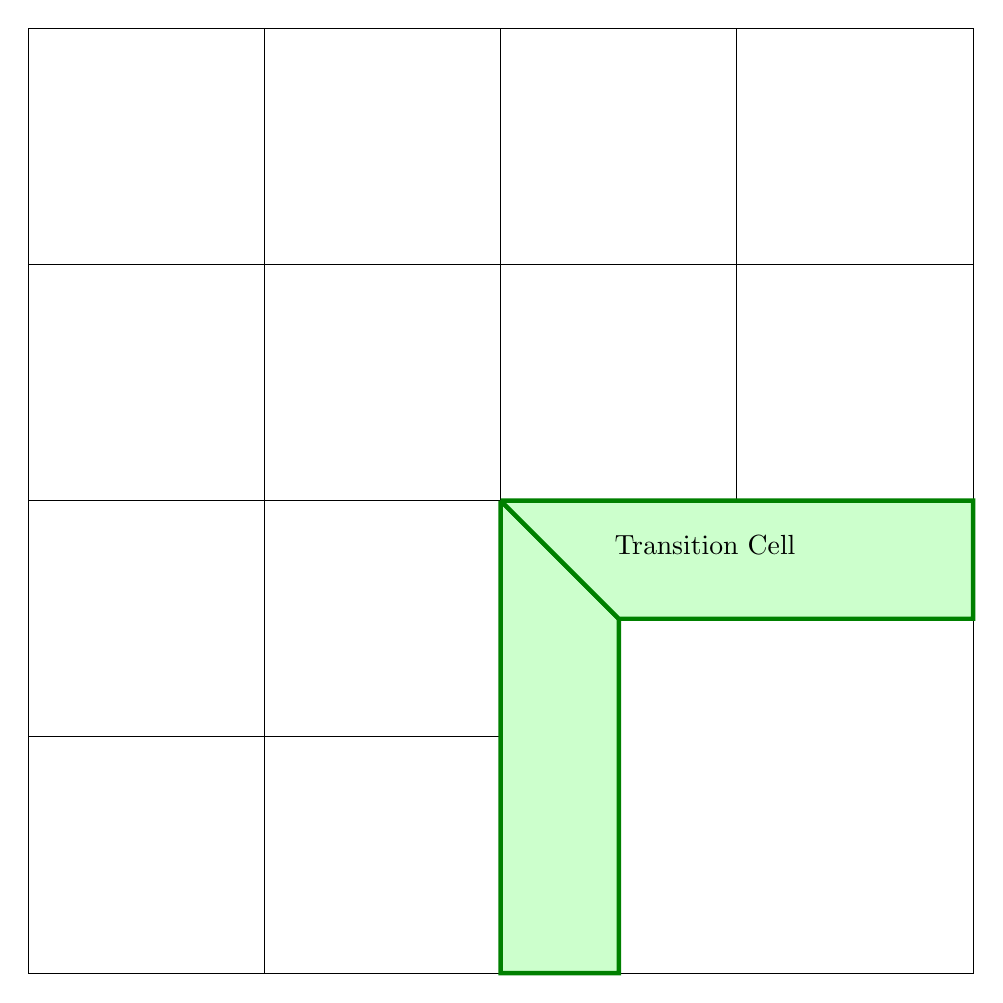
\begin{tikzpicture}[scale=3]
  \draw (0, 0) rectangle (1, 1);
  \draw (1, 0) rectangle (2, 1);
  \draw (0, 1) rectangle (1, 2);
  \draw (1, 1) rectangle (2, 2);

  \draw (2, 2) rectangle (3, 3);
  \draw (3, 2) rectangle (4, 3);
  \draw (2, 3) rectangle (3, 4);
  \draw (3, 3) rectangle (4, 4);

  \draw (0, 2) rectangle (1, 3);
  \draw (1, 2) rectangle (2, 3);
  \draw (0, 3) rectangle (1, 4);
  \draw (1, 3) rectangle (2, 4);

  \draw (2.5, 0) rectangle (4, 1.5);

  \begin{scope}[ultra thick]
    \filldraw[fill=green!20!white, draw=green!50!black] (2, 2) -- (2, 0) -- (2.5, 0) -- (2.5, 1.5) -- (2, 2);
    \filldraw[fill=green!20!white, draw=green!50!black] (2, 2) -- (4, 2) -- (4, 1.5) -- (2.5, 1.5) -- (2, 2) node [below=1.6em, right=3.7em] {Transition Cell};
  \end{scope}
\end{tikzpicture} \\ \\

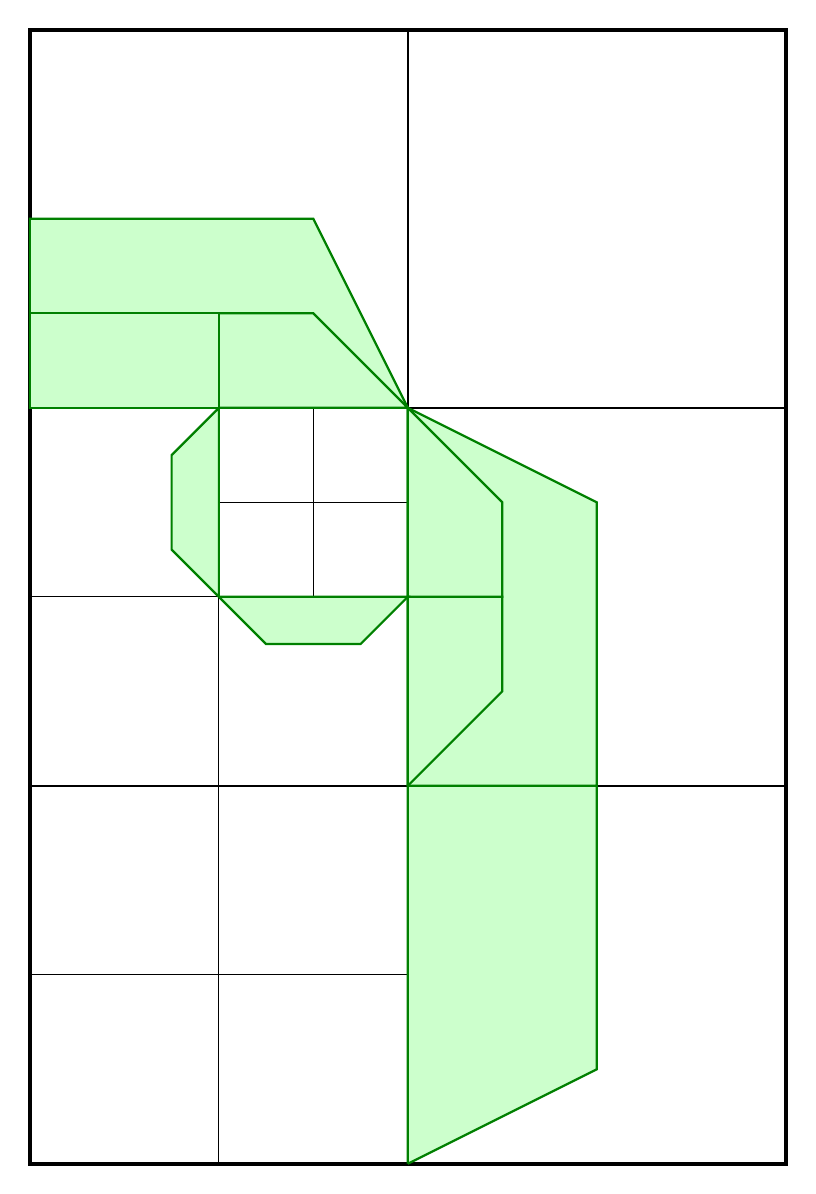
\begin{tikzpicture}[scale=1.2]
  % Draw a border around the quadtree figure
  \begin{scope}[ultra thick]
    \draw (0, 0) rectangle (8, 12);
  \end{scope}
  % Draw the quadtree nodes at three levels
  \begin{scope}[thick]
    \draw (0, 0) rectangle (4, 4);
    \draw (4, 0) rectangle (8, 4);
    \draw (0, 4) rectangle (4, 8);
    \draw (4, 4) rectangle (8, 8);
    \draw (0, 8) rectangle (4, 12);
    \draw (4, 8) rectangle (8, 12);
  \end{scope}
  \begin{scope}
    \draw (0, 0) rectangle (2, 2);
    \draw (2, 0) rectangle (4, 2);
    \draw (0, 2) rectangle (2, 4);
    \draw (2, 2) rectangle (4, 4);

    \draw (0, 4) rectangle (2, 6);
    \draw (2, 4) rectangle (4, 6);
    \draw (0, 6) rectangle (2, 8);
    \draw (2, 6) rectangle (4, 8);
  \end{scope}
  \begin{scope}[very thin]
    \draw (2, 6) rectangle (3, 7);
    \draw (3, 6) rectangle (4, 7);
    \draw (2, 7) rectangle (3, 8);
    \draw (3, 7) rectangle (4, 8);
  \end{scope}
  % Draw the transition cells, being careful to draw the larger ones first
  \begin{scope}[fill=green!20!white, draw=green!50!black, thick]
    % Large transitions
    \filldraw (4, 0) -- (6, 1) -- (6, 4) -- (4, 4) -- (4, 0);
    \filldraw (4, 4) -- (6, 4) -- (6, 7) -- (4, 8) -- (4, 4);
    \filldraw (4, 8) -- (3, 10) -- (0, 10) -- (0, 8) -- (4, 8);
    % Small transitions
    \filldraw (4, 4) -- (5, 5) -- (5, 6) -- (4, 6) -- (4, 4);
    \filldraw (4, 6) -- (5, 6) -- (5, 7) -- (4, 8) -- (4, 6);
    \filldraw (4, 8) -- (3, 9) -- (2, 9) -- (2, 8) -- (4, 8);
    \filldraw (0, 8) -- (2, 8) -- (2, 9) -- (0, 9) -- (0, 8);
    % Smallest transitions
    \filldraw (2, 6) -- (2.5, 5.5) -- (3.5, 5.5) -- (4, 6) -- (2, 6);
    \filldraw (2, 6) -- (1.5, 6.5) -- (1.5, 7.5) -- (2, 8) -- (2, 6);
  \end{scope}
\end{tikzpicture}
}
\subcolumn{0.5}
\block{42 Regular Cell Cases}{Blocktext}
\block{72 Transition Cell Cases}{Blocktext}
\end{subcolumns}
\end{columns}
\end{document}
